%*****************************************
\chapter{Ergebnisse}\label{ch:results}
%*****************************************

\section{Vergleich der Ergebnisse des HMM sowie des CRF}

% Please add the following required packages to your document preamble:
% \usepackage{booktabs}
% \usepackage{graphicx}
\begin{table}[]
\centering
\caption{Genauigkeit der beiden Modelle über beide Durchläufe. Durchlauf 2 Zeigt den Effekt des Trainings des CRF.}
\label{tab:accuracy-results}
\resizebox{\textwidth}{!}{%
\begin{tabular}{@{}lllllll@{}}
\toprule
Modell                                                       & blood & low\_quality & nbi   & outside & polyp  & Insgesamt \\ \midrule
\begin{tabular}[c]{@{}l@{}}HMM -\\ Durchlauf 1\end{tabular}  & 0,0   & 0,489        & 0,010 & 0,977   & 0,0067 & 0,331     \\
\begin{tabular}[c]{@{}l@{}}HMM - \\ Durchlauf 2\end{tabular} & 0     & 0,480        & 0,008 & 0,974   & 0,0067 & 0,328     \\
\begin{tabular}[c]{@{}l@{}}CRF -\\ Durchlauf 1\end{tabular}  & 0,270 & 0,491        & 0,217 & 0,966   & 0,156  & 0,427     \\
\begin{tabular}[c]{@{}l@{}}CRF -\\ Durchlauf 2\end{tabular}  & 0,439 & 0,708        & 0,012 & 0,960   & 0,156  & 0,511     \\ \bottomrule
\end{tabular}%
}
\end{table}

\begin{table}[htbp]
\centering
\caption{Laufzeitanalyse (inkl.\ Feature-Extraktion und Diffusion) auf 500 Frames.}
\label{tab:timing-summary}
\resizebox{\textwidth}{!}{%
\begin{tabular}{@{}llll@{}}
\toprule
Bereich & Kennzahl & HMM & CRF \\ \midrule

\multicolumn{4}{@{}l@{}}{\textbf{Gesamt}} \\
Frames verarbeitet & Anzahl & 500 & 500 \\
Laufzeit & Wall-clock & 23{,}18\,s & 23{,}18\,s \\
Durchsatz & FPS & 21{,}6 & 21{,}6 \\ \midrule

\multicolumn{4}{@{}l@{}}{\textbf{Feature-Extraktion (ms)}} \\
Mittelwert & mean   & 34{,}50 & 34{,}50 \\
Median    & median & 31{,}09 & 31{,}09 \\
Perzentil & p90    & 44{,}08 & 44{,}08 \\
Minimum   & min    & 29{,}47 & 29{,}47 \\
Maximum   & max    & 180{,}99 & 180{,}99 \\ \midrule

\multicolumn{4}{@{}l@{}}{\textbf{Inferenzzeiten (ms)}} \\
Mittelwert & mean   & 0{,}03 & 0{,}16 \\
Median    & median & 0{,}03 & 0{,}14 \\
Perzentil & p90    & 0{,}04 & 0{,}22 \\
Minimum   & min    & 0{,}03 & 0{,}12 \\
Maximum   & max    & 0{,}11 & 1{,}03 \\ \midrule

\multicolumn{4}{@{}l@{}}{\textbf{Gesamt pro Frame (ms)}} \\
Mittelwert & mean   & 34{,}53 & 34{,}69 \\
Median    & median & 31{,}13 & 31{,}28 \\
Perzentil & p90    & 44{,}11 & 44{,}25 \\
Minimum   & min    & 29{,}50 & 29{,}64 \\
Maximum   & max    & 181{,}03 & 181{,}20 \\ \bottomrule
\end{tabular}%
}
\end{table}



% Please add the following required packages to your document preamble:
% \usepackage{booktabs}
\begin{table}[]
\centering
\caption{Präzision, Recall und F1 über alle Videos.}
\label{tab:vergleich_alle_videos}
\resizebox{\textwidth}{!}{%
\begin{tabular}{@{}llrrrr@{}}
\toprule
Modell & Label & Precision & Recall & F1 & Support \\ \midrule
HMM & blood & 0{,}00\% & 0{,}00\% & 0{,}00\% & 27902 \\
CRF & blood & 30{,}49\% & 43{,}91\% & 35{,}99\% & 27902 \\ \midrule
HMM & low\_quality & 81{,}42\% & 48{,}02\% & 60{,}41\% & 57733 \\
CRF & low\_quality & 65{,}98\% & 70{,}81\% & 68{,}31\% & 57733 \\ \midrule
HMM & nbi & 1{,}76\% & 0{,}86\% & 1{,}15\% & 9435 \\
CRF & nbi & 12{,}47\% & 1{,}16\% & 2{,}11\% & 9435 \\ \midrule
HMM & outside & 44{,}38\% & 97{,}42\% & 60{,}98\% & 32312 \\
CRF & outside & 59{,}98\% & 96{,}04\% & 73{,}84\% & 32312 \\ \midrule
HMM & polyp & 48{,}47\% & 0{,}67\% & 1{,}33\% & 54333 \\
CRF & polyp & 50{,}29\% & 15{,}63\% & 23{,}85\% & 54333 \\ \midrule
\multicolumn{2}{@{}l}{Macro F1} & \multicolumn{1}{r}{0{,}138} & \multicolumn{1}{r}{--} & \multicolumn{1}{r}{0{,}227} & \multicolumn{1}{r}{--} \\
\multicolumn{2}{@{}l}{Micro F1} & \multicolumn{1}{r}{0{,}328} & \multicolumn{1}{r}{--} & \multicolumn{1}{r}{0{,}511} & \multicolumn{1}{r}{--} \\ \bottomrule
\end{tabular}%
}
\end{table}


\section{Analyse der Ergebnisse des Vergleichs von HMM und CRF}

Die Modelle wurden zuerst 

Die Eingangs beschriebenen Modelle unterscheiden sich vor allem in einem Punkt: Während das HMM mit Kalman-Diffusion ohne Training die wahrscheinlichste Abfolge aus den Features schätzt, nutzt das CRF gelernte Gewichte für die existierenden Featurefuntionen. Aus diesem Grund ist die Erwartung, dass sich die Performance des CRF mit dem Training verbessert.

\section{Diskussion der Ergebnisse und Implikationen für die Systemarchitektur}

Die quantitative Auswertung der HMM- und CRF-Modelle offenbart eine signifikante Dichotomie in der Klassifikationsleistung, die für das Design einer effizienten Analyse-Pipeline von entscheidender Bedeutung ist. Während die Modelle bei der Differenzierung pathologischer Befunde (insbesondere \textit{polyp} vs. \textit{blood}) deutliche Schwächen zeigen – was sich in einer Polyp-Erkennungsrate von unter 25\,\% selbst im besten CRF-Szenario widerspiegelt, demonstrieren sie Robustheit bei der Identifikation irrelevanter Videosequenzen.

Insbesondere die Klassen \textit{outside} - Frames außerhalb des Videos wurden mit einer Genauigkeit von bis zu 98\,\%  korrekt klassifiziert. Frames mit dem label \textit{low\_quality} - Frames mit schlechter Bildqualität - wurden  Die Analyse der Konfusionsmatrizen legt nahe, dass die verwendeten farbbasierten Merkmale ausreichen, um technische Artefakte und extrakorporale Aufnahmen zuverlässig von organischem Gewebe zu trennen.

\begin{figure}[htbp]
    \centering
    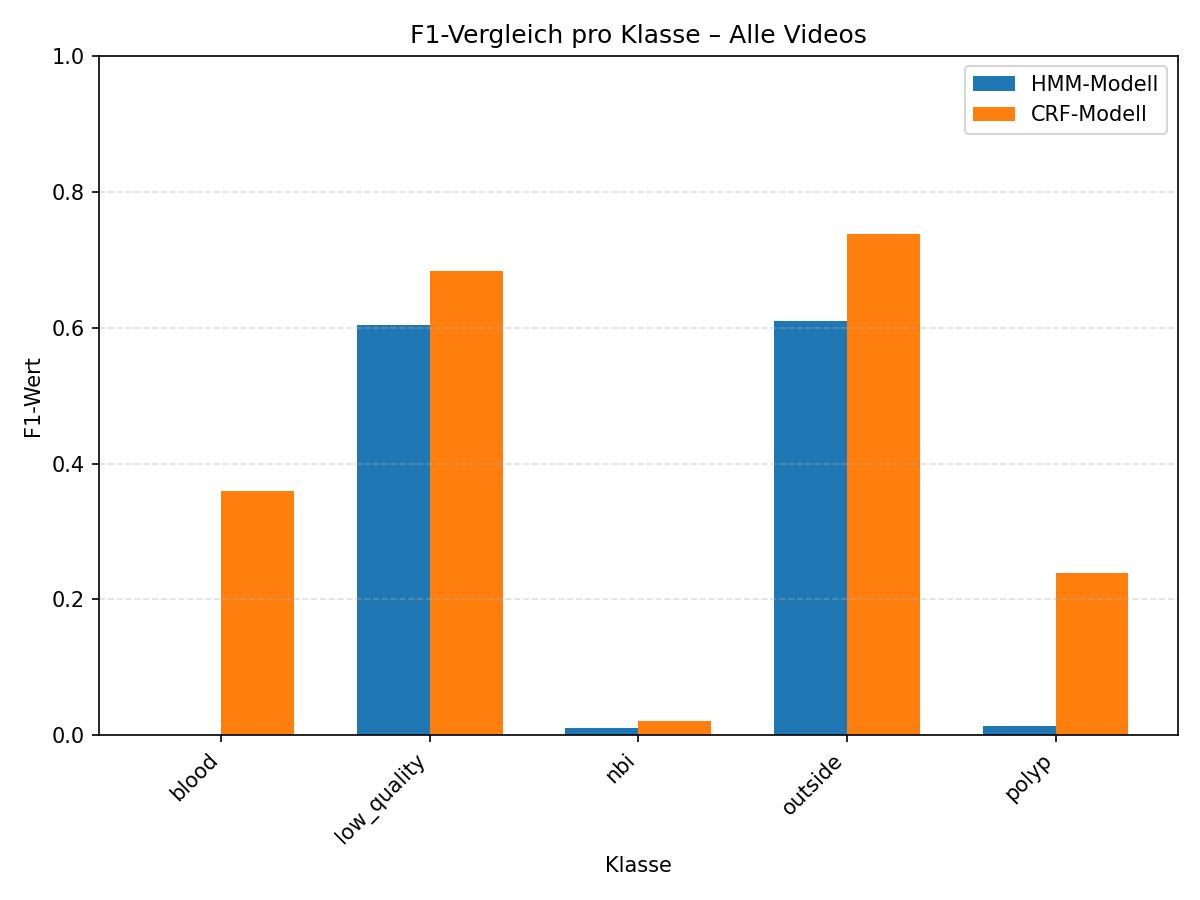
\includegraphics[width=0.9\textwidth]{Images/vergleich_Alle_Videos.png}
    \caption{Vergleich der Modellleistung über alle Videos.}
    \label{fig:vergleich_alle_videos}
\end{figure}

\paragraph{Interpretation der F1-Scores.}
Da das vorliegende Datenset eine starke Klassenimbalance aufweist, ist die alleinige Betrachtung der Genauigkeit nur eingeschränkt aussagekräftig. Der F1-Score, als harmonisches Mittel aus Precision und Recall, erlaubt eine robustere Bewertung der Klassifikationsleistung, da er sowohl Fehlklassifikationen als auch verpasste Erkennungen berücksichtigt.

Für das HMM zeigt sich, dass mehrere Klassen – insbesondere \textit{blood} und \textit{polyp} – praktisch nicht erkannt werden (F1 nahe $0$), obwohl die Gesamtgenauigkeit durch dominante Klassen wie \textit{outside} relativ hoch ausfällt. Dies spiegelt die Limitierung eines rein regelbasierten, generativen Modells wider, dessen Übergangsdynamik seltene Zustände unterdrücken kann.

Das CRF erreicht durch das Training der Übergangsgewichte signifikant höhere F1-Werte in nahezu allen Klassen. Besonders für \textit{outside} (F1 $=73{,}84\%$) und \textit{low\_quality} (F1 $=68{,}31\%$) wird eine robuste Balance zwischen Precision und Recall erzielt. Für pathologische Klassen wie \textit{polyp} und \textit{blood} verbessert sich der F1-Score deutlich gegenüber dem HMM, verbleibt jedoch unterhalb eines für eine alleinige diagnostische Nutzung ausreichenden Niveaus.

Der Vergleich von Macro- und Micro-F1 verdeutlicht diese Beobachtung: Während der Micro-F1 des CRF ($0{,}511$) einen substantiellen Gesamtgewinn belegt, bleibt der Macro-F1 ($0{,}227$) begrenzt. Dies zeigt, dass das Modell insbesondere für häufige und klar separierbare Klassen zuverlässig arbeitet, während seltene oder visuell komplexe Zustände weiterhin eine Herausforderung darstellen.

Diese Beobachtung motiviert den Einsatz eines kaskadierten Systemansatzes, welches das Filtern der Frames mit dem CRF mit dem Einsatz anderer Modelle zu kombinieren. Die stochastischen Modelle qualifizieren sich aufgrund ihrer geringen Inferenzzeit (ca. 30\,ms pro Frame) ideal als Vorfilterstufe. In einer kombinierten Pipeline übernimmt das CRF-Modell die Rolle eines \textit{Gatekeepers}, der den Datenstrom effizient um nicht-diagnostische Frames bereinigt. Der verbleibende, signifikant reduzierte Datenbestand kann anschließend an ein leistungsstärkeres, aber rechenintensiveres Convolutional Neural Network (CNN) oder an ein Vison Transformer Modell übergeben werden. Durch diese Arbeitsteilung lässt sich die Effizienz des Systems steigern, indem die Ressourcen des CNNs gezielt auf die schwierigen pathologischen Unterscheidungen fokussiert werden, während das CRF die Echtzeitfähigkeit des Systems durch schnelle Vorselektion gewährleistet.
